\documentclass[11pt]{article}
\usepackage[a4paper,margin=2.2cm]{geometry}
\usepackage{amsmath,amssymb}
\usepackage{booktabs}
\usepackage{tikz}
\usepackage{xcolor}
\usepackage{caption}
\usepackage{float}
\usepackage{tabularx}
\captionsetup{font=small,labelfont=bf}

\definecolor{spect}{gray}{0.6}
\definecolor{move}{RGB}{200,30,30}

% \lvl{x}{y}{name}{electrons}{colour}: one orbital level with 0, 1 or 2 electrons
\newcommand{\lvl}[5]{%
  \draw[thick,#5] (#1-0.45,#2) -- (#1+0.45,#2);
  \node[anchor=west,font=\footnotesize,#5] at (#1+0.5,#2) {$#3$};
  \ifnum#4>0 \draw[-latex,#5] (#1-0.12,#2-0.17) -- (#1-0.12,#2+0.19);\fi
  \ifnum#4>1 \draw[-latex,#5] (#1+0.12,#2+0.19) -- (#1+0.12,#2-0.17);\fi
}
% core-valence gap
\newcommand{\gap}[2]{\draw[dashed,spect] (#1-0.7,#2) -- (#1+0.95,#2);}

\title{Shake-down cases: general orbital roles}
\author{XPSoverlaps}
\date{}

\begin{document}
\maketitle
\vspace{-2em}

\section{Orbital roles}

An initial state $a$ is a single excitation $i\to k$ from the closed-shell reference.
A shake-down goes to a lower-energy initial state $b$ that differs from $a$ by one
moved electron; the core-ionised final state $\Phi^F$ has the valence occupation of $b$
and one electron removed from the core orbital $c$. The roles are defined by
occupation in the reference, not by a fixed HOMO/LUMO assignment:

\medskip\noindent
\begin{tabularx}{\textwidth}{@{}l>{\raggedright\arraybackslash}Xll@{}}
\toprule
Label & Role & Reference occupation & Physical orbital \\
\midrule
$c$ & core; doubly occupied initially, singly finally & occupied (core) & e.g.\ S\,2p \\
$i$ & pump hole: emptied by the pump & occupied & HOMO$-n$, $n\ge 0$ \\
$k$ & pump particle: filled by the pump & virtual & LUMO$+m$, $m\ge 0$ \\
$j$ (3e ES) & receives the shake-down electron & virtual, below $k$ & LUMO$+l$, $l<m$ \\
$j$ (5e ES) & gives the shake-down electron; doubly occupied in $a$ & occupied, above $i$ & HOMO$-n'$, $n'<n$ \\
$d$ & HOMO when it is none of $i, j$; doubly occupied throughout & occupied & HOMO \\
\bottomrule
\end{tabularx}
\medskip


The spectator $d$ carries no spin and is left out of the rules. Energy order:
3e cases $\varepsilon_i<\varepsilon_d<\varepsilon_j<\varepsilon_k$;
5e case $\varepsilon_i<\varepsilon_j<\varepsilon_d<\varepsilon_k$.

\section{Which case applies}

The case is set by \emph{where the shake-down electron comes from}, read off by comparing
$b$ with $a$ (both written as excitations from the reference):

\begin{center}
\begin{tabular}{@{}lll@{}}
\toprule
$b$ compared with $a=(i\to k)$ & Shake-down electron & Case \\
\midrule
$b$ is the reference & $k\to i$, from the virtual $k$ into the hole & 3e GS \\
same hole $i$, lower particle & $k\to j$, from the virtual $k$ into a lower virtual & 3e ES \\
same particle $k$, different hole & $j\to i$, from a doubly occupied $j$ into the hole & 5e ES \\
\bottomrule
\end{tabular}
\end{center}

Only one row can hold for a given pair, so an initial HOMO$-n\to$LUMO$+m$ state usually
has several shake-downs, each with its own case. The 5e rules are needed only when an
electron leaves an orbital that was \emph{doubly occupied} in $a$; whenever the moving
electron is the pumped one in $k$, the 3e rules apply.

\section{Configurations}

Figure~\ref{fig:cases} shows the occupations for each case; in short:

\begin{figure}[tb]
\centering
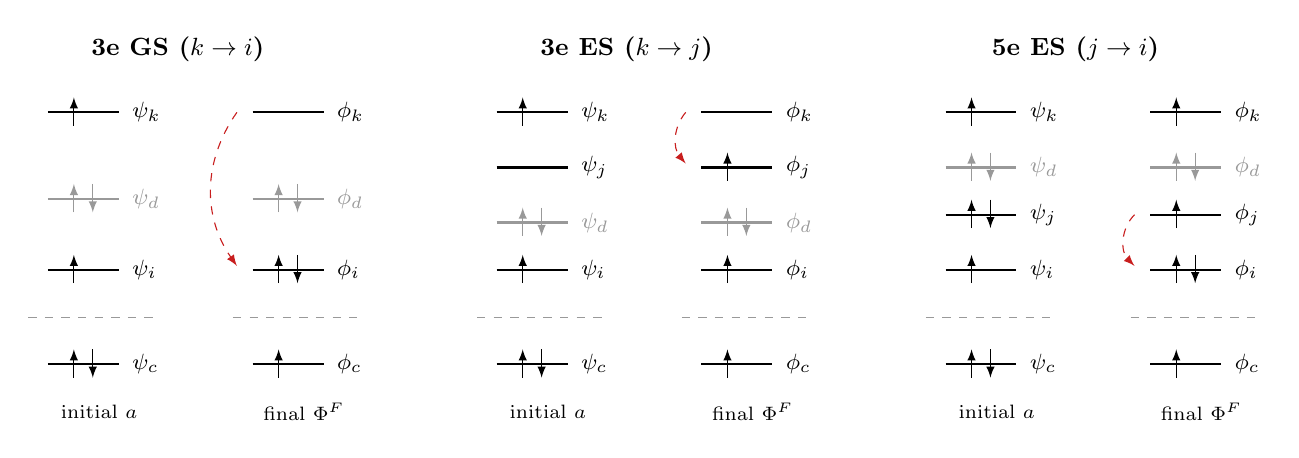
\begin{tikzpicture}
  % ---- 3e GS
  \begin{scope}[shift={(0,0)}]
    \node[font=\small\bfseries] at (1.2,4.0) {3e GS ($k\to i$)};
    \gap{0}{0.6} \lvl{0}{0}{\psi_c}{2}{black}
    \lvl{0}{1.2}{\psi_i}{1}{black} \lvl{0}{2.1}{\psi_d}{2}{spect} \lvl{0}{3.2}{\psi_k}{1}{black}
    \node[font=\scriptsize] at (0.2,-0.6) {initial $a$};
    \gap{2.6}{0.6} \lvl{2.6}{0}{\phi_c}{1}{black}
    \lvl{2.6}{1.2}{\phi_i}{2}{black} \lvl{2.6}{2.1}{\phi_d}{2}{spect} \lvl{2.6}{3.2}{\phi_k}{0}{black}
    \draw[-latex,dashed,move] (1.95,3.2) to[bend right=35] (1.95,1.25);
    \node[font=\scriptsize] at (2.8,-0.6) {final $\Phi^F$};
  \end{scope}
  % ---- 3e ES
  \begin{scope}[shift={(5.7,0)}]
    \node[font=\small\bfseries] at (1.2,4.0) {3e ES ($k\to j$)};
    \gap{0}{0.6} \lvl{0}{0}{\psi_c}{2}{black}
    \lvl{0}{1.2}{\psi_i}{1}{black} \lvl{0}{1.8}{\psi_d}{2}{spect}
    \lvl{0}{2.5}{\psi_j}{0}{black} \lvl{0}{3.2}{\psi_k}{1}{black}
    \node[font=\scriptsize] at (0.2,-0.6) {initial $a$};
    \gap{2.6}{0.6} \lvl{2.6}{0}{\phi_c}{1}{black}
    \lvl{2.6}{1.2}{\phi_i}{1}{black} \lvl{2.6}{1.8}{\phi_d}{2}{spect}
    \lvl{2.6}{2.5}{\phi_j}{1}{black} \lvl{2.6}{3.2}{\phi_k}{0}{black}
    \draw[-latex,dashed,move] (1.95,3.2) to[bend right=40] (1.95,2.55);
    \node[font=\scriptsize] at (2.8,-0.6) {final $\Phi^F$};
  \end{scope}
  % ---- 5e ES
  \begin{scope}[shift={(11.4,0)}]
    \node[font=\small\bfseries] at (1.2,4.0) {5e ES ($j\to i$)};
    \gap{0}{0.6} \lvl{0}{0}{\psi_c}{2}{black}
    \lvl{0}{1.2}{\psi_i}{1}{black} \lvl{0}{1.9}{\psi_j}{2}{black}
    \lvl{0}{2.5}{\psi_d}{2}{spect} \lvl{0}{3.2}{\psi_k}{1}{black}
    \node[font=\scriptsize] at (0.2,-0.6) {initial $a$};
    \gap{2.6}{0.6} \lvl{2.6}{0}{\phi_c}{1}{black}
    \lvl{2.6}{1.2}{\phi_i}{2}{black} \lvl{2.6}{1.9}{\phi_j}{1}{black}
    \lvl{2.6}{2.5}{\phi_d}{2}{spect} \lvl{2.6}{3.2}{\phi_k}{1}{black}
    \draw[-latex,dashed,move] (1.95,1.9) to[bend right=45] (1.95,1.25);
    \node[font=\scriptsize] at (2.8,-0.6) {final $\Phi^F$};
  \end{scope}
\end{tikzpicture}
\caption{\label{fig:cases}Occupations of the initial state $a$ and the core-ionised final state $\Phi^F$
(valence as in $b$) for each case. Red: the shake-down electron. Grey: the HOMO spectator
$d$, present only when it is none of $i,j$ (i.e.\ $i$ = HOMO$-n$ in 3e, $j\ne$ HOMO in 5e);
otherwise $d$ is absent and the diagram is unchanged. Dashed line: core--valence gap.}
\end{figure}

\begin{center}
\small
\begin{tabular}{@{}llll@{}}
\toprule
Case & Initial $a$ & Final $\Phi^F$ & Lower initial state $b$ \\
\midrule
3e GS & $\psi_c^2\,\psi_i^1\,(\psi_d^2)\,\psi_k^1$ & $\phi_c^1\,\phi_i^2\,(\phi_d^2)$ & reference \\
3e ES & $\psi_c^2\,\psi_i^1\,(\psi_d^2)\,\psi_k^1$ & $\phi_c^1\,\phi_i^1\,(\phi_d^2)\,\phi_j^1$ & $i\to j$ \\
5e ES & $\psi_c^2\,\psi_i^1\,\psi_j^2\,(\psi_d^2)\,\psi_k^1$ & $\phi_c^1\,\phi_i^2\,\phi_j^1\,(\phi_d^2)\,\phi_k^1$ & $j\to k$ \\
\bottomrule
\end{tabular}
\end{center}

\section{Rules}

$S_{ab}=|\langle\phi_a|\psi_b\rangle|$, where $\phi_a$ is the final-state orbital that the
orbital mapping matches to initial orbital $a$. CVS: $S_{cc}=1$, $S_{ca}=S_{ac}=0$.
Diagonal overlaps are set to $S_{ii}=S_{jj}=S_{kk}=1$; the code reports any whose actual
value is below 0.9.

\begin{center}
\begin{tabular}{@{}lll@{}}
\toprule
& 3e (GS, ES) & 5e ES \\
\midrule
$\Pi$ (direct) & $S_{jk}$ & $M_1M_2$ \\
$\Omega$ (exchange) & $S_{ik}S_{ji}$ & $M_3M_4$ \\
Singlet $\to D_1$ & $|\Pi+\Omega|^2$ & $|\Pi+\Omega|^2$ \\
Triplet channels & $|\Pi-\Omega|^2\times$ spin weight & $|\Pi-\Omega|^2\times$ spin weight \\
GS shake-down & $2|S_{ik}|^2$ & --- \\
\bottomrule
\end{tabular}
\end{center}
with $M_1=1-S_{ij}S_{ji}$, $M_2=S_{ij}-S_{ik}S_{kj}$, $M_3=S_{ij}S_{jk}-S_{ik}$,
$M_4=S_{kj}-S_{ij}S_{ki}$. The GS shake-down uses $2|S_{ik}|^2$ for every pump, including
HOMO$-n$ pumps ($d$ omitted).

\section{Not computed}

\begin{itemize}\setlength\itemsep{0pt}
\item $a$ or $b$ is a double excitation: no rule.
\item The electron would move up ($\varepsilon_j>\varepsilon_k$ in 3e ES, or the donor below
  the hole in 5e ES).
\item The order cannot be checked: with only HOMO and LUMO known, 3e ES needs $j$ = LUMO
  and 5e ES needs $j$ = HOMO; other pairs are reported as ``orbital order unknown''.
\end{itemize}

\section{Example}

Bromothiophene, S\,2p core hole; HOMO = mo:34, LUMO = mo:40.

\begin{center}
\small
\begin{tabular}{@{}llllllll@{}}
\toprule
$a\to b$ & $a$ & $b$ & Electron & Case & $i$ & $j$ & $k$ ($d$) \\
\midrule
$2\to1$ & mo:34$\to$40 & reference & 40$\to$34 & 3e GS & 34 & -- & 40 \\
$5\to1$ & mo:38$\to$41 & reference & 41$\to$38 & 3e GS & 38 & -- & 41 (34) \\
$5\to3$ & mo:38$\to$41 & mo:38$\to$40 & 41$\to$40 & 3e ES & 38 & 40 & 41 (34) \\
$5\to4$ & mo:38$\to$41 & mo:34$\to$41 & 34$\to$38 & 5e ES & 38 & 34 & 41 \\
$6\to5$ & mo:37$\to$41 & mo:38$\to$41 & 38$\to$37 & 5e ES & 37 & 38 & 41 (34) \\
\bottomrule
\end{tabular}
\end{center}
State 5 shows one pump with three shake-downs of different cases. $6\to5$ is a 5e ES with
$j$ = HOMO$-1$; it is computable once the order of mo:37 and mo:38 is known.

\end{document}
